\hsection{Basics of Classes}%
%
We learned about simple datatypes in \cref{sec:simplyDataTypesAndOperations}.
We then also got to know different kinds of collections, i.e., datatypes that can hold multiple elements, in \cref{sec:collections}.
However, in many situations, we deal with data that cannot satisfyingly represented by either of them alone.
Many datatypes are compound structures of different elements that are semantically related to each other.
For example, a the elements of a list or tuple are related only in the sense that they appear in the same collection.
If we look at a \emph{date} however, then there is a much more meaningful relationship between its components \emph{day}, \pythonil{month}, and \pythonil{year}.
Such datatypes and the operations on them also often form a semantic unit.

Imagine, for example, you would like to implement mathematical operations for complex numbers.\footnote{%
\python\ already offers the datatype \pythonilIdx{complex} for this purpose, but for the sake of the example, assume it does not.}
Of course, you could represent complex numbers as \pythonil{tuple[float, float]}.
This, however, comes with several drawbacks.

On one hand, not \emph{every} tuple of two \pythonils{float} is to be understood as a complex number.
So just from the \pgls{signature} of your functions, i.e., just based on its parameters and return types, it is not immediately clear that your functions are for complex numbers.
All we can directly see is that they are for tuples of two \pythonils{float}.

On the other hand, the two parts of a complex numbers, the real part and the imaginary part, have two distinct and different meanings.
It would not immediately be clear whether the first number of the tuple is the real or the imaginary part.
Indeed, we could also represent complex numbers in polar form, in which case the two tuple elements would have yet different meanings.
Also, the standard textual representation of tuples of two \pythonils{float} would be something like~\pythonil{"(3.0, 4.0)"}, whereas we would probably prefer something like~\pythonil{"3+4i"} for complex numbers.

The first important use-cases of \pythoniles{class} in \python\ is that they offer us a way to define a data structure together with the operations for it as one semantic unit~\cite{PSF:P3D:TPT:C}.
This allows us to define a \pythonil{class} for complex numbers which has attributes with the names \pythonil{real_part} and \pythonil{imaginary_part}.
We can define operators like addition and subtraction that work with instances of this \pythonil{class}, making it immediately clear how and when they are to be used.
And this \pythonil{class} can then have default textual representations of our liking.

A second situation where ability to define functions and we have learned so far hits a limit arises with \pglspl{API} that have different implementations.
Let us be ambitious and imagine that you wanted to create a versatile system that can produce documents.
On the output side, you want to support different formats, say \libreoffice~\cite{DF2024LTDF,GL2012LTSOOSSCBAFACSOL}, \microsoftWord~\cite{MS2024MW,DR2019STFAWAUMW}, and Adobe~\pgls{formatPDF}~\cite{A2024WDPM,A2008P3DMPDFP1P1}.
On the input side, you would like to provide the user/programmer with a uniform way to create documents.

This input side \pgls{API} should be the same for all output formats.
It would not just consist of a single function, but several groups of functions.
There could even be nested hierarchies of operations that you would like to support, e.g., the add chapters, paragraphs, and maybe runs of text in different fonts.
Obviously, these operations will be implemented differently for the different output formats.

We could try to solve this by making different modules for different output formats.
Each modul could contain functions of the same name and \pglspl{signature}, realizing the required behaviors.
But this would be a huge hassle.
The bibbest problem would be that there would be no way to define a central blueprint of \inQuotes{how the \pgls{API} looks like.}
It can easily lead to inconsistencies during the software life cycle.
If we slightly change the \pgls{signature} of one function, we need to implement this in all of the modules.
There also is no way that a \pgls{linter} like \ruff\ could tell is if some module is no longer synchronized due to the lack of a central blueprint.

Classes offer us the necessary abstraction.
We could specify a base class \pythonil{Document} for document objects that provides methods for the necessary operations, from adding text to aligning figures.
These operations could just \pythonilIdx{raise} a \pythonilIdx{NotImplementedError}.
Then, for each output format, we could derive a new subclass from this base class with the actual implementation of the methods.
The code on the user side could treat all these different document types the same, because all of them would be instances of \pythonil{Document} with the same operations.
The format-specific stuff would all be invisible to the user, exactly as it should be.
\Pglspl{linter} then can also tell us if one certain implementation of the subclass does not correctly adher to the \pgls{API} defined in the base class.
So the second important use case for classes are that they offer us a very nice abstraction for defining and implementing \pglspl{API}.

Classes therefore can solve two important problems where the basic datatypes, collections, and plain functions we learned about are not sufficient:
First, they allow us to semantically and clearly group data and operations together.
Second, they offer us a simple way to group several operations into one \pgls{API}, which then -- transparently to the user -- can be implemented in different ways.
In this chapter, we discuss \pythoniles{class} in \python.
Syntactly, \pythoniles{classes} follow the general blueprint below~\cite{PSF:P3D:TPT:C}.%
%
\pythonSyntax{syntax/class_init_method.py}%
\FloatBarrier%
%
Classes are datatypes that combine data elements with the code working on them~\cite{PSF:P3D:TPT:C}.
A class is basically a blueprint or a concept, whereas objects are the concrete instances of the classes.
For example \pythonil{int} is basically a class of integer numbers, whereas \pythonil{5} is an instance of this class.

Classes are declared with the keyword \pythonil{class} followed by the class name, followed by a colon~(\inQuotes{:}).
The class body is then indented by four spaces.
It contains everything that belongs to the class, including the documentation, methods, and attributes.
The first item after the class declaration is usually the \pgls{docstring} of the class.
It can be a single descriptive line or a multi-line documentation, in which case it begins with a single summary line, followed by an empty line, followed by the comprehensive documentation text.
%
\bestPractice{className}{\sloppy%
Class names should follow the CapWords convention~(often also called \emph{camel case}), i.e., look like \pythonil{MyClass} or \pythonil{UniversityDepartment} (not \pythonil{my_class} or \pythonil{university_department})~\cite{PEP8}.}%
%
A class can have a initializer method \dunder{init}.
This special method can take arbitrarily many parameters, but never returns a value.
It is annotated with \pglspl{typeHint} and with a \pgls{docstring} like a normal function.
Only the special parameter \pythonilIdx{self} is not annotated.

The initializer \dunder{init} is used to declare all of the classes'~(non-inherited) instance attributes by assigning them their initial values.
We also provide attribute \pglspl{typeHint} in this step.
In all methods of the class, the current object/instance of the class is referenced by the name~\pythonilIdx{self}.
If we access an attribute or a method of a class, we always use the prefix~\pythonil{self.}.
We therefore always declare \pythonilIdx{self} as the first parameter of every method.
Thus, a line like \pythonil{self.x: int = 5} in \dunder{init}, creates the instance attribute \pythonil{x}, type-hints it as integer, and assigns to it the initial value~5.
We can put a short comment describing the meaning of the attribute in the line \emph{before} its declaration.
This comment will always have a colon right after the hash, i.e. always begins with \pythonil{\#: }\cite{SD2024SIDFD:DCAD}.
For example, writing \pythonil{\#: This is the x-coordinate.} in the line before the declaration of an attribute \pythonil{self.x} would annotate this attribute with documentation stating that it is, well, an \glslink{xAxis}{x}-coordinate.

Classes can have arbitrarily many methods.
A method is a function that works on or with the attributes of a class instance.
Each such method has as first parameter \pythonilIdx{self}, denoting the object instance of the class the method works on.
A method can have arbitrarily many other parameters and, if you want, also a return value.
All parameters except \pythonil{self} are of course annotated with \pglspl{typeHint}.
Methods also have \pglspl{docstring}, like normal functions.
In the method, we can access the both the attributes and methods of the instance again via the \pythonil{self.}-prefix.

After defining the class, we can now instantiate it.
For this, we use the class name like a normal function.
We need to provide arguments, i.e., values, for all parameters of \dunder{init} except \pythonilIdx{self}.
We can use objects of this class like normal values, and, e.g., store them in variables.
We can also use the class name as a \pgls{typeHint}, because it represents a normal type.

So much about the general structure of \pythoniles{class}.
Now, without further ado, let's explore this structure with some examples.%
%
\hsection{Design Principle: Immutable Classes}%
\label{sec:immutableClassPoints2D}%
%
\gitLoadPython{classes:point}{}{classes/point.py}{}%
\listingPython{classes:point}{%
A class for representing points in the two-dimensional Euclidean plane}%
%
\gitLoadAndExecPython{classes:point_user}{}{classes}{point_user.py}{}%
\listingPythonAndOutput{classes:point_user}{%
An example of using our new class \pythonil{Point} from \cref{lst:classes:point}.}{}%
%
We begin directly with an example.
Assume that we want to write a program that processes points in the two-dimensional Euclidean plane.
Every point is defined by its x\nobreakdashes~and y\nobreakdashes-coordinate.
We could use a \pythonil{tuple} of two numbers, say a~\pythonil{tuple[int | float, int | float]}, to represent such points.
This is totally fine and a quick solution.

However, this solution lacks semantics, i.e., it lacks a clear and obvious meaning.
There is nothing that says that a \pythonil{tuple[int | float, int | float]} must be a point in the two-dimensional Euclidean plane.
It could just as well be a tuple of travel time and an associated cost for a train ride from Hefei to Beijing, taken from the train schedule of a particular day.
Basically, it just is a grouping of two numbers.
The same lack of semantics appears when we try to implement operations that process our points.
A function that computes the distance between two such points would just take two \pythonils{tuple} as input.
Of course, I should pass in only \pythonils{tuple} that actually represent points in the two-dimensional plane.
But nothing really can stop me from passing in other tuples, such as \pythonils{tuple} holding the travel times and associated costs for train rides from Hefei to Beijing.
Of course, the results would probably not make any sense.
Yet, such situations may arise from misunderstandings or lack of documentation.

In the ideal case, if I am working with points in the two-dimensional Euclidean plane, then I have a data structure that clearly and unambiguously is designed for such points and such points only.
The operations for the points should only accept instances of this data structure as input~(and raise\pythonIdx{raise} exceptions\pythonIdx{Exception} if fed something else as arguments).
If I am accessing the x\nobreakdashes-coordinate of a point, it should be absolutely clear from the semantics and names involved that this is, indeed, the x\nobreakdashes-coordinate and not something else, not just the first number of a \pythonil{tuple} of two numbers.

Such clear semantics can be achieved with \pythoniles{class}\pythonIdx{class} in \python.
In \cref{lst:classes:point}, you can find exactly this example as file \programUrl{classes:point}.
We create the class \pythonil{Point}\pythonIdx{class} by writing \pythonil{class Point:}.
We then create the class body, which we indent by four spaces.
Of course the first thing we place in the class body is always a \pgls{docstring}.%
%
\bestPractice{classDocString}{%
At the beginning of a \pythonilIdx{class}, a \pgls{docstring} is placed which describes what the class is good for. %
This \pgls{docstring} can include \pglspl{doctest} to demonstrate the class usage. %
Such \pglspl{doctest} can also be placed in the \pgls{docstring} of the module.%
}%
%
Afterwards, we will place all the \emph{methods} of the \pythonilIdx{class} in the class body.
Methods are like functions, but their first parameter is always called \pythonilIdx{self} and always is an instance of the class, i.e., an object.
Either way, all these methods go into the class block.

Our class \pythonil{Point} will have two attributes, \pythonil{x} and~\pythonil{y}.
A attribute is a variable that every single instance of the class has.
We later want to be able to create one instance of \pythonil{Point} with the x\nobreakdashes-coordinate~5 and the y\nobreakdashes-coordinate~10 and then another instance with the x\nobreakdashes-coordinate~2 and the y\nobreakdashes-coordinate~7.
So each instance of \pythonil{Point} needs to have these two attributes.

Therefore, \pythonil{Point} needs a initializer, i.e., a special method that creates and initializes these attributes.
This method is called~\dunder{init}.
As said, every method of a class must have a parameter~\pythonilIdx{self}, which is the instance of the class~(the object) upon which the method is called.
The initializer \dunder{init} is a special method, so it also has this parameter~\pythonilIdx{self}.
Additionally, we demand that values for the two parameters~\pythonil{x} and~\pythonil{y} be passed in when we create an instance of~\pythonil{Point}.
We allow the values to be either \pythonils{int} or \pythonils{float}.

Inside every method of a class, the attributes of objects are accessed via the parameter~\pythonilIdx{self}.
We can read the attribute~\pythonil{x} of an object inside a method of the class by writing~\pythonil{self.x}.
Here, \pythonil{self.x} can be used just like a normal local variable.
We can store the value~\pythonil{a} in a (mutable) attribute~\pythonil{x} of the current object in a method of the class by writing~\pythonil{self.x = a}.
This value will then remain the same until it is changed in exactly that way, even after the execution of the method is completed.%
%
\bestPractice{attributes}{%
Object attributes must only be created inside the initializer~\dunder{init}. %
There, an initial value must immediately be assigned to each attribute.%
}
%
We only want to allow \pythonils{Point} that have finite coordinates.
As explained in the \cref{sec:exceptions} on \pythonilsIdx{Exception}, it is better to immediately signal errors if we encounter invalid data.
So we want to sort out non-finite coordinates right when someone attempts to create the \pythonil{Point} object.
Thus, the first thing we do in the initializer is to use the \pythonilIdx{isfinite} function from the \pythonilIdx{math} module.
If either \pythonil{x} or \pythonil{y} is not finite, then we raise\pythonIdx{raise} a \pythonilIdx{ValueError}.\footnote{%
Strictly speaking, it could also make sense to check whether \pythonil{x} and \pythonil{y} are indeed either \pythonil{int} or \pythonil{float}. %
For example, we could check if \pythonil{isinstance(x, int | float)}\pythonIdx{isinstance} and this is \pythonil{False}, raise\pythonIdx{raise} a~\pythonilIdx{TypeError}. %
However, that would make the example overly long, so I am not doing this here.%
}

Otherwise, we set \pythonil{self.x: Final[int | float] = x} and \pythonil{self.y: Final[int | float] = y}.
These lines create the attributes \pythonil{self.x} and \pythonil{self.y} of the object which was passed in via the parameter~\pythonil{self}.
The \pgls{typeHint} \pythonilIdx{Final} from the \pythonilIdx{typing} module annotates a variable or attribute as immutable~\cite{PEP591}.
In other words, we do not allow the coordinates of our \pythonils{Point} to change after object creation.%
%
\bestPractice{attributeTypeHint}{%
Every attribute of an object must be annotated with a \pgls{typeHint} when created in the initializer~\dunder{init}~\cite{LM2024WTMD}. %
Here, \pglspl{typeHint} work exactly like with normal variables.}%
%
\bestPractice{attributeFinal}{%
The \pgls{typeHint} \pythonilIdx{Final}\pythonIdx{typing!Final} marks a variable or attribute as immutable. %
All attributes that you do not intend to change should be annotated with~\pythonilIdx{Final}\pythonIdx{typing!Final}. %
Notice that this is a \pgls{typeHint}, i.e., it will not be enforced by the \python\ interpreter~\cite{PEP591} and malicious code can \emph{still} change the attribute value. %
Type checkers like \mypy\ can detect such incorrect changes, though, and issue warnings.%
}%
%
We will explore this issue a bit later in detail.%
%
\bestPractice{attributeDocstring}{%
An attribute is documented in the line \emph{above} the attribute initialization by writing a \emph{comment} starting with \pythonilIdx{\#: }, which explains the meaning of the attribute~\cite{SD2024SIDFD:DCAD}. %
(Sometimes, the documentation is given as string directly below the attribute definition~\cite{PEP287}, but we stick to the former method, because it has proper tool support, e.g., by~\sphinx.)%
}%
%
After properly defining our initializer, we can now do something like~\pythonil{p = Point(1, 2)}.
This creates a new object as an instance of our \pythonilIdx{class} \pythonil{Point}.
Therefore, first, the necessary memory for~\pythonil{p} is allocated.
Then, the initializer is invoked as~\pythonil{\_\_init\_\_(p, 1, 2)}.
After the initializer is completed, the object is stored in the varible, i.e., \pythonil{p} now refers to a \pythonil{Point}~object.
The attribute \pythonil{p.x} has the value~\pythonil{1} and \pythonil{p.y} has value~\pythonil{2}.

From the knowledge that \pythonil{p} is an instance of \pythonil{Point}, we can immediately see that \pythonil{p.x} and \pythonil{p.y} are its x-\ and y\nobreakdashes-coordinate, respectively.
There is no way to mistake the meaning of these variables.
Of course, our \pglspl{docstring} with \pglspl{doctest} and the \pglspl{typeHint} further help the reader to understand their meaning.

Having a new class for points in the two-dimensional plane is already nice.
But such a \pythonil{class} also allows us to define operations on points in form of methods.
As an example, we implement a method \pythonil{distance} that computes the distance between two points.
You would have a point~\pythonil{p1} and invoke \pythonil{p1.distance(p2)} to compute the distance to another point~\pythonil{p2}.
The computation itself will follow \cref{eq:euclideanDistance} from our recent endeavor to operations on iterations in \cref{sec:operationsOnIterators}.
We therefore need to import the \pythonilIdx{sqrt} function from the \pythonilIdx{math} module.

Our new method \pythonil{distance} will have two parameters, \pythonilIdx{self}, which will be the object upon which we invoke the method~(\pythonil{p1}~in the above example) and~\pythonil{p}, the other object~(or \pythonil{p2} above).
It then just has to compute the Euclidean distance~\pythonil{sqrt((self.x - p.x) ** 2 + (self.y - p.y) ** 2)}.
Inside a method of an object, \pythonilIdx{self} always refers to the object itself.
Therefore, \pythonil{self.x}~is the x\nobreakdashes-coordinate of the current object and \pythonil{self.y}~is its~y\nobreakdashes-coordinate.
\pythonil{p.x}~is the x\nobreakdashes-coordinate of the point~\pythonil{p} that was passed in as actual parameter of the method, and \pythonil{p.y}~is its y\nobreakdashes-coordinate.
Notice that the \pgls{docstring} not just explains how this method is used, but also provides a simple example in form of a~\pgls{doctest}.
If you compute \pythonil{Point(1, 1).distance(Point(4, 4))}, then the expected result is something like~4.243{\dots}%
%
\begin{sloppypar}%
In this \pgls{doctest} -- \pythonil{Point(1, 1).distance(Point(4, 4))} -- we only provided a single parameter to the method~\pythonil{distance}.
When calling the method~\pythonil{distance}, we never need to provide a value of the parameter~\pythonilIdx{self} directly.
Instead, it will be provided indirectly:
If we have two points~\pythonil{p1} and~\pythonil{p2} and invoke~\pythonil{p1.distance(p2)}, then~\pythonil{self = p1} will be set automatically.
Hence, even though we declared our method as~\pythonil{def distance(self, p: \"Point\") -> float}, which looks as if we need to provide two parameters~(\pythonilIdx{self} and~\pythonil{p}), we only need to provide one, namely~\pythonil{p}.%
\end{sloppypar}%
%
Reading this again, we notice that the parameter~\pythonil{p} is annotated with a very strange \pgls{typeHint}:
One would expect that we would annotate it with~\pythonil{Point}, instead it is annotated with the string~\pythonil{\"Point\"}.
This has the simple reason that the complete class \pythonil{Point} is only defined \emph{after}, well, the complete definition of class~\pythonil{Point}.
Therefore, \pythonil{Point} is not yet available as type \emph{inside} its definition.
Using the string~\pythonil{\"Point\"} here is therefore just a crutch with no real other effect.
%
%
\bestPractice{methodDocstring}{%
All methods of \pythoniles{class} must be annotated with \pglspl{docstring} and \pglspl{typeHint}.%
}%
\bestPractice{ownClassTypeHint}{%
When using a class~\pythonil{C} as \pgls{typeHint} \emph{inside} the definition of the class~\pythonil{C}, you must write~\pythonil{"C"} instead of~\pythonil{C}. %
(Otherwise, static code analysis tools and the \python\ interpreter get confused.)%
}%
%
We could now go on and add more methods that do reasonable computations with instances of~\pythonil{Point}.
For now, this simple example will suffice.
Let us instead take a look on how one would use our new class with program \programUrl{classes:point_user} given as \cref{lst:classes:point_user}.

Before we can do anything, we need to import our class \pythonil{Point}.
Class \pythonil{Point} is defined in file \programUrl{classes:point}.
The file name without the \textil{.py} is the module name~(\pythonil{point}) from where we can import the class.
Hence, we write \pythonil{from point import Point}.

We now can create one instance of~\pythonil{Point} and store it in a variable~\pythonil{p1}.
Since~\pythonil{p1} is supposed to reference an instance of~\pythonil{Point}, its \pgls{typeHint} should denote this.
Here we can use \pythonil{Point} just like any other datatype.
We write \pythonil{p1: Point = Point(3, 5)}.
The initializer \dunder{init} is automatically invoked when we write~\pythonil{Point(3, 5)}.
The two arguments that we pass in will be provided to it as values for parameters~\pythonil{x} and~\pythonil{y}, respectively.
The first parameter, \pythonilIdx{self}, of \dunder{init} will be a newly allocated and yet un-initialized instance of \pythonil{Point}.

After \dunder{init} completes, the resulting new instance of \pythonil{Point} that we get should have its attribute~\pythonil{x} set to~\pythonil{3} and its attribute~\pythonil{y} set to~\pythonil{5}.
We can access them via~\pythonil{p1.x} and~\pythonil{p1.y}.
Of course we can also use them in an \pgls{fstring}.
We find that \pythonil{f\"\{p1.x = \}, \{p1.y = \}\"} will be \glslink{strinterpolation}{interpolated} to \pythonil{\"p1.x = 3, p1.y = 5\"}.

The type of \pythonil{p1} is \pythonil{Point}.
The class \pythonil{Point} is defined in file \programUrl{classes:point}.
This file name is interpreted as module name~\pythonil{point}.
Hence, the full name of the type is \pythonil{point.Point}.
And it is a \pythonilIdx{class}.
Hence, printing \pythonil{type(p1)}\pythonIdx{type} yields \textil{<class \'point.Point\'>}.

We can check if an object~\pythonil{o} is an instance of our class \pythonil{Point} by writing~\pythonil{isinstance(o, Point)}\pythonIdx{isinstance}.
For \pythonil{p1}, this returns~\pythonil{True}, as one would expect.
As a test, we check whether \pythonil{isinstance(5, Point)}, which returns \pythonil{False} for similarly obvious reasons.
\pythonil{isinstance(p1, int)} is \pythonil{False}, too.

We now create a second instance, \pythonil{p2}, of the class \pythonil{Point}.
We this time, just for fun, pass the arguments by parameter name, i.e., write \pythonil{x=8} and \pythonil{y=7}.
These arguments will then again be passed to \dunder{init}.
This assigns \pythonil{7} to \pythonil{p2.x} and \pythonil{8} to \pythonil{p2.y}.
We can again print the values of these attributes using an \pgls{fstring}.

The \pythonilIdx{type} of \pythonil{p2} is again the \pythonilIdx{class} \pythonil{point.Point}.
Our objects can be used with the \pythonilIdx{is}~operator, which checks for object identity.
\pythonil{p1}~is the same object as itself, which means that \pythonil{p1 is p1}\pythonIdx{is} yields~\pythonil{True}.
While being instances of the same class, \pythonil{p1} and \pythonil{p2} are different objects.
Therefore, \pythonil{p1 is p2}\pythonIdx{is} yields~\pythonil{False}.
%
\begin{sloppypar}%
We can now also use our method \pythonil{distance}.
\pythonil{p1.distance(p2)}, i.e., the distance from~\pythonil{p1} to~\pythonil{p2}, is the same as \pythonil{p2.distance(p1)}, i.e., the distance from~\pythonil{p2} to~\pythonil{p1}.
Both are equal to~5, because~$\sqrt{(7 - 3)^2 + (8 - 5)^2}=\sqrt{4^2 + 3^2}=\sqrt{25}=5$.%
\end{sloppypar}%
%
\pythonil{Point} can indeed be used like any other datatype that we discussed before.
For example, we can have lists of instances of \pythonils{Point}.
The appropriate \pgls{typeHint} for such a list would be \pythonil{list[Point]}.
We can even create such a list with list comprehension\pythonIdx{list!comprehension}\pythonIdx{comprehension!list}, exactly as we learned back in \cref{sec:listComprehension}.

We can then process this list by writing a generator expression which transforms the points to strings, just as we discussed in \cref{sec:generatorExpressions}.
The expression interpolates the \pgls{fstring} \pythonil{f\"(\{p.x\}, \{p.y\})\"} for each \pythonil{Point} \pythonil{p} in our list \pythonil{point_list}.
This means that a sequence of strings of the form \textil{\"(x, y)\"} is created.
These are then concatenated by the \pythonilIdx{join}\pythonIdx{str!join} method of the string~\pythonil{\", \"}~(see \cref{sec:loopsOverSequences}).
The result can be seen at the bottom of \cref{exec:classes:point_user}.

\pythonil{Point} is a datatype like any other datatype.
Actually, it is the very first datatype in \python\ that we have created.
This is quite cool, if you think about it.
The programming language has datatypes like \pythonil{str} or \pythonil{list}.
Now we are now able to extend the programming language with our own datatypes, that make sense in our own scenarios.

The objects of our \pythonil{Point} class are \emph{immutable}.
Once created, the attributes cannot be changed anymore, at least not without violating the language rules.
The thing that (should) stop anyone from changing them is the \pythonilIdx{Final} \pgls{typeHint}.
As said before, in \python, \pglspl{typeHint} are just hints and not enforced by the interpreter~\cite{PEP591}.
Thus, the attributes \pythonil{x} and \pythonil{y} of instances of \pythonil{Point} can actually be changed.
However, tools like \mypy\ will detect such mistakes and report them~\cite{PEP591}.%

\gitLoadAndExecPython{classes:point_user_wrong}{}{classes}{point_user_wrong.py}{}%
\listingPythonAndOutput{classes:point_user_wrong}{%
An example program that uses our new class \pythonil{Point} incorrectly: %
We violate the \pythonilIdx{Final} annotation of attribute~\pythonil{x} by overwriting it.}{}%
%
\begin{figure}%
\centering%
\tightbox{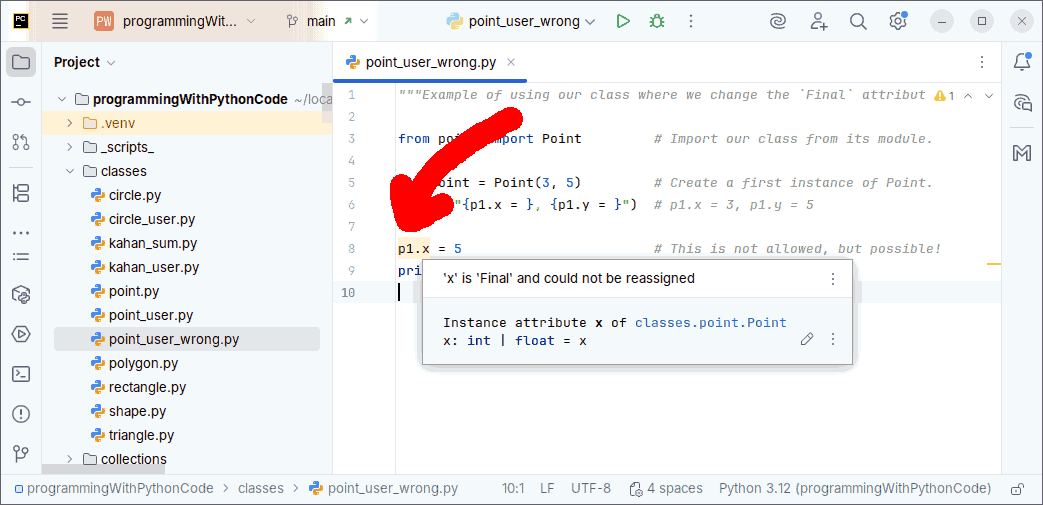
\includegraphics[width=0.7\linewidth]{\currentDir/finalViolatedPycharm}}%
\caption{%
We open our program \programUrl{classes:point_user_wrong} from \cref{lst:classes:point_user_wrong} that uses the class \pythonil{Point} incorrectly in \pycharm. %
If we hover the mouse over the yellow mark in the line that violates the \pythonilIdx{Final} annotation, \pycharm\ informs us that doing that is wrong.}%
\label{fig:finalViolatedPycharm}%
\end{figure}%
%
\gitExec{exec:classes:point_user_wrong:mypy}{\programmingWithPythonCodeRepo}{.}{_scripts_/mypy.sh classes point_user_wrong.py}%
\listingToolOutput{classes:point_user_wrong:mypy}{%
The result of applying \mypy\ to the program \programUrl{classes:point_user_wrong} from \cref{lst:classes:point_user_wrong} that violates the \pythonilIdx{Final} annotation of the attributes of our class \pythonil{Point}. %
\mypy\ reports the issue.}%

Program \programUrl{classes:point_user_wrong} explores this problem in \cref{lst:classes:point_user_wrong}.
After creating the \pythonil{Point} object~\pythonil{p1} exactly as in our first example, it frivolously sets \pythonil{p1.x = 5}.
The \pythonilIdx{Final} \pgls{typeHint} tells us explicitly that this should not be done.
However, as the output in \cref{exec:classes:point_user_wrong} shows, we can do it anyway.

That this is not a good idea becomes already clear when we open our program in \pycharm.
\Cref{fig:finalViolatedPycharm} illustrates that \pycharm\ highlights the violating line of code with a yellow mark.
Hovering the mouse over this note tells us in no uncertain terms that we are doing something that should be forbidden.
\mypy\ gives us a similar warning in \cref{exec:classes:point_user_wrong:mypy}.

The attributes \pythonil{x} and \pythonil{y} are initialized by \dunder{init}.
There, they are also marked with the \pgls{typeHint} \pythonilIdx{Final} and thus changing them is an error.
But why did we do that?
Why did we start this topic so early when delving into classes?
Because in many cases, making objects immutable is a good design pattern.%
%
\cquotation{B2008EJ}{%
Classes should be immutable unless there's a very good reason to make them mutable{\dots}.
If a class cannot be made immutable, limit its mutability as much as possible.%
}%
%
\begin{definition}[Immutable]%
After their initialization, the attributes of \emph{immutable} objects cannot be modified anymore.%
\end{definition}%
%
Creating classes whose instances are immutable has several benefits, e.g.:
Code gets easier to understand, because we do not need to think about whether, when, or how an object changes (because it cannot).
The elements of sets and the keys of dictionaries in \python, for example, must be immutable objects because these collection store objects based on their hash codes which, in turn, are based on the attributes of these objects.
If the attributes would change, so would the hash codes, which means that the objects could no longer be found.
Immutable objects are especially useful in parallel programming, where mutable shared state could lead to complex bugs and race conditions.

Still, there also are many cases where we want to create objects whose attributes can change.
We will explore one of them in the next section.

But before we do that, let's summarize what we have learned and practically played with so far:
By defining our own classes, we can create our own data structures.
We can use classes just like any other datatype.

Classes can have their own variables, which are called attributes.
They also can have associated functions, which are called methods.
The methods access the attributes to compute stuff.
Each class can have arbitrarily many attributes and methods.

A special method is the initializer \dunder{init}.
It is called automatically when we create a new instance of the class.
Here, all the attributes of a class instance created and receive their initial value.

Of course, we use \pglspl{typeHint} and \pglspl{docstring} as well as \pglspl{doctest} also with classes.
For example, ee can mark attributes as immutable with the \pythonilIdx{Final} \pgls{typeHint}.
Sadly, \python\ does not strictly enforce that, i.e., we can technically still change \pythonilIdx{Final} attributes.
This, however, is a sin that luckily is detected by tools like \mypy\ and even \pglspl{ide} like \pycharm.
Marking attributes as immutable is still a good idea, because it prevents many possible bugs.%
\FloatBarrier%
\endhsection%
%
\hsection{Design Principle: Encapsulation}%
\FloatBarrier%
%
\gitEvalPython{classes:adding_floats_error}{}{classes/adding_floats_error.py}%
\listingBox{exec:classes:adding_floats_error}{%
Computations with \pythonil{float} that hit the digit limit, which explored back in \cref{sec:howFloatingPointNumbersWork}.}{,style=python_console_style}%
%
We often want our objects to be immutable.
This obviously cannot always be the case.
There also are many situations, where we need objects whose state can change.
Then the question is \emph{How should the state of an object be changed?}
The vast majority of our classes will have more than one instance attributes.
All the attributes of an object together make up its state and form a semantic unit.

If an object has multiple attributes, these attributes may be inter-related and their values depent on each other.
We would not want that somebody can change the attributes willy-nilly.
Often we want to design mutable objects such that the values of their mutable attributes can only be accessed via methods.
The methods and attributes of a class from a semantic unit, too.
The methods are written by the same programmer(s) who designed the attributes.
These programmers know exactly how the attributes can be changed in a consistent and meaningful way.

We now explore exactly such a secario.
We have a class whose attributes are tightly inter-related, such that it would not make any sense to allow a user to change them separately.
Instead, we implement methods that can change the attributes in a consistent way and query information from the object.
Of course, being the math nerds we are, we will do this on the example of a mathematical algorithm.

We already implemented some interesting mathematical algorithms.
We implemented the method of LIU Hui~(刘徽) for approximating~\numberPi\ in \cref{sec:approximatePiLiuHui}, Heron's Method for approximating the square root in \cref{sec:whileLoop}, and Euclid's algorithm for the greatest common divisor in \cref{sec:definingFunctions}.
All of these algorithms you likely have seen in high school.
Let's now implement an algorithm that you probably never heard about:
A practical method that tries to mitigate the limitations of the datatype \pythonil{float}, that we discussed way back in \cref{sec:float}.

We learned that the datatype \pythonilIdx{float} can represent numbers accurately to about 15 to 16 digits.
This is illustrated in \cref{exec:classes:adding_floats_error}:
If we add~\pythonil{1} to~$10^{15}=\pythonil{1e15}$, the correct result is~\pythonil{1000000000000001.0}.
As you can count, there are 16 digits before the decimal dot, two~\pythonils{1} and 14~\pythonils{0}.
Consequenly, adding~\pythonil{1} to~$10^{16}=\pythonil{1e16}$ would require 17~digits.
This exceeds the capacity of our \pythonils{float}.
Hence, the least-significant digit just \inQuotes{falls off.}
The result of \pythonil{1e16 + 1} computed mit \pythonils{float} is still~\pythonil{1e16}.
It is not possible to represent the number~$1+10^{16}$ exactly with the 64~bit double precision floating point numbers that \python\ offers~\cite{PSF:P3D:TPT:FPAIAL,IEEE2019ISFFPA,H1997IS7FPN}.

Usually, that itself is totally fine:
There are only very few application were we really need more than 15 digits of precision.
Still, let's continue this example for a bit.
What happens if we try to compute~$10^{18}+1$ and then subtract~$10^{18}$ from this sum?
Obviously, in an ideal world, the result should be~\pythonil{1.0}.
While \pythonil{1e16 + 1} would be \pythonil{10_000_000_000_000_001.0} which does not fit in a \pythonil{float}, \pythonil{1.0}~is a number that we can correctly and accurately represent as a~\pythonilIdx{float}.
The actual result of this computation in \python, however, is~\pythonil{0.0}.
The reason is that the result of the intermediate computation of \pythonil{1e18 + 1 == 1e18} and then \pythonil{1e18 - 1e18 == 0}.

Similarly, computing \pythonil{1e18 + 1 + 1e36 - 1e36 - 1e18} yields~\pythonil{-1e18}, while the \inQuotes{correct} result would again be~\pythonil{1.0}.
The reason is that first, \pythonil{1e18 + 1 == 1e18} is computed.
Then \pythonil{1e18 + 1e36} yields~\pythonil{1e36}, from which we subtract~\pythonil{1e36} and get~\pythonil{0.0}.
The final subtraction of~\pythonil{1e18} then results in~\pythonil{1e-18}.
If we had infinite precision, the first step would instead yield~$10^{18}+1=1\decSep000\decSep000\decSep000\decSep000\decSep000\decSep001$
Adding \pythonil{1e36} to this number should then yield~$1000\decSep000\decSep000\decSep000\decSep000\decSep001\decSep000\decSep000\decSep000\decSep000\decSep000\decSep001$.
Subtracting~\pythonil{1e36} from this humongous number would bring us back to~$10^{18}+1$ and the final subtraction of~\pythonil{1e18} would give us~\pythonil{1.0}.
It is easy to see why this does not work out.
The designers of the floating point number arithmetic unit in CPUs had to choose some limited number of bits per \pythonil{float}.
They concluded that 52~bits of \pgls{significand} giving us $52/\log_2 10\approx 15.7$~digits are reasonable and neatly fit into a 8~bytes of memory.
On the other hand, 36~digits, requiring a \pgls{significand} of $36\log_2 10\approx 120$~bits, would make the datatype much bigger and are probably never actually needed.
Well, never, unless you try to add up large and small numbers.

The interesting question that we may ask after reviewing the example is:
\emph{Is there a way to more accurately add large and small numbers?}
Of course, we can never represent \pythonil{1e16 + 1} exactly as \pythonil{float}.
However, we want to be able to represent the final result of a sum at least as accurately as possible.
For example, we want a way to compute the sum \pythonil{(1e18 + 1) + -1e18} such that the result is \pythonil{1.0}.
Is this possible?

Luckily, in the 1960s, \citeauthor{K1965PFRORTE}~\cite{K1965PFRORTE} and \citeauthor{B1968NSIMA}~\cite{B1968NSIMA} had an idea how to extend the precision of additions~\cite{G1991WECSSKAFPA,L2020RWECSSKAFPA}:
We add numbers up in a \pythonil{sum} variable and carry with us a variable~\pythonil{cs} where we remember how far off this sum is.
Imagine again that we want to compute \pythonil{1e18 + 1 - 1e18}.
How could we do that to arrive at the result~\pythonil{1.0}?
By following this simple algorithm that maintains the overall sum of the numbers in a variable~\pythonil{sum} and keeps track of an error term in a variable~\pythonil{cs}:%
%
\begin{enumerate}%
%
\item We start with \pythonil{sum = 0} and \pythonil{cs = 0}.%
%
\item For each number to add to the sum, we perform the following steps:%
\begin{enumerate}%
%
\item We first compute \pythonil{t = sum + value}. %
\pythonil{t}~thus is the sum as precisely as a \pythonil{float} can represent it.
%
\item We then calculate~\pythonil{error = (sum - t) + value}. %
Since \pythonil{t = sum + value}, we could assume that \pythonil{error} should be~\pythonil{0.0}, because it looks as if it effectively is~\pythonil{(sum - (sum + value)) + value}. %
However, some digits could have been \inQuotes{lost} when computing \pythonil{sum + value}.
They will re-appear in \pythonil{error}.%
%
\item We then set \pythonil{sum = t}.%
%
\item We accumulate the errors in~\pythonil{cs}, i.e., set~\pythonil{cs += error}.%
%
\end{enumerate}%
%
\item The final result of the summation is then \pythonil{sum + cs}.
\end{enumerate}%
%
In the example \pythonil{1e18 + 1 - 1e18}, we have three numbers that we want to sum up.
Let's follow through with this simple algorithm above.%
%
\begin{enumerate}%
\item We start with \pythonil{sum = 0} and \pythonil{cs = 0}.%
%
\item The first number that we want to add to the sum is \pythonil{1e18}.%
\begin{enumerate}%
\item In the first step, we have to compute~\pythonil{t = sum + value}, i.e., \pythonil{t = 0 + 1e18}, meaning that~\pythonil{t = 1e18}.%
%
\item Then, \pythonil{error = (sum - t) + value} becomes \pythonil{error = (0 - 1e18) + 1e18}, which gives us~\pythonil{error = 0.0}.%
\item We set~\pythonil{sum = t}, also \pythonil{sum = 1e18}.%
\item \pythonil{cs}, which was~\pythonil{0}, becomes \pythonil{0 + 0.0}, which means that it now is~\pythonil{cs = 0.0}.%
\end{enumerate}%
%
\item The second number that we want to add to the sum is \pythonil{1}.%
\begin{enumerate}%
%
\item We compute~\pythonil{t = sum + value}. %
Now this mean~\pythonil{t = 1e18 + 1} and this results in~\pythonil{t = 1e18}. %
The~\pythonil{1} is lost.%
%
\item Well, almost: %
\pythonil{error = (sum - t) + value} becomes \pythonil{error = (1e18 - 1e18) + 1}, i.e., \pythonil{error = 1.0}.%
%
\item After this step, \pythonil{sum = 1e18}.%
%
\item And \pythonil{cs = 0 + 1.0} becomes~\pythonil{1.0}.%
\end{enumerate}%
%
\item We now subtract~\pythonil{1e18} from the sum, which is equivalent to adding~\pythonil{-1e18}.%
%
\begin{enumerate}%
\item This means that we first compute~\pythonil{t = sum + value}, i.e., \pythonil{t = 1e18 + -1e18}, which leads us to~\pythonil{t = 0.0}.%
%
\item For the error term, we get \pythonil{error = (1e18 - 0.0) + -1e18}, which leads to~\pythonil{error = 0.0}.%
%
\item We now got~\pythonil{sum = 0.0}.%
%
\item And~\pythonil{cs = 1.0 + 0.0}, which still means that~\pythonil{cs = 1.0}.%
\end{enumerate}%
%
\item The final result will be~\pythonil{sum + cs} and this indeed gives us~\pythonil{0.0 + 1.0}, i.e., \pythonil{1.0}!
%
\end{enumerate}%
%
Although we cannot represent the intermediate results of the addition exactly, we still got the right result.
With the \citeauthor{K1965PFRORTE}-Sum, we can compute the correct result of \pythonil{1e18 + 1 - 1e18}, namely~\pythonil{1.0}.
The trick was to keep track of the total error in the variable~\pythonil{cs}.
The price thus is that we needed additional variables and needed to update them in each step.%
%
\FloatBarrier%
%
\insertAlgorithm{kahanSum}{%
The second-order \citeauthor{K1965PFRORTE}-\citeauthor{B1968NSIMA}-\citeauthor{N1974REVZSES} summation algorithm~\cite{B1968NSIMA,K1965PFRORTE,N1974REVZSES,K2006AGKBSA} over an array~\aVar{x} of $n$~numbers as defined by~\citeauthor{K2006AGKBSA} in~\cite{K2006AGKBSA}.}{%
%
\aAssign{\aVar{sum}}{0}\aSep%
\aAssign{\aVar{cs}}{0}\aSep%
\aAssign{\aVar{ccs}}{0}\algoCmtEndline{Initialze sum, 1st order- and 2nd order error.}%
%
\For(\algoCmtInline{For each of the $n$ numbers to add.}){$\aVar{i} \in \intRange{0}{n-1}$}{%
\aAssign{\aVar{t}}{\aVar{sum}+\aArrayIndex{\aVar{x}}{\aVar{i}}}\algoCmtEndline{Compute the sum and (below) the first-order error term~\cite{B1968NSIMA,K1965PFRORTE}.}%
\lIf(\algoCmtInline{the tweak by \citeauthor{N1974REVZSES}~\cite{N1974REVZSES}}){$|\aVar{sum}|\geq|\aArrayIndex{\aVar{x}}{\aVar{i}}|$}{%
\aAssign{\aVar{c}}{(\aVar{sum}-\aVar{t})+\aArrayIndex{\aVar{x}}{\aVar{i}}}%
}\lElse{%
\aAssign{\aVar{c}}{(\aArrayIndex{\aVar{x}}{\aVar{i}}-\aVar{t})+\aVar{sum}}%
}%
%
\aAssign{\aVar{sum}}{\aVar{t}}\algoCmtEndline{The overall sum is updated.}%
\aAssign{\aVar{t}}{\aVar{cs}+\aVar{c}}\algoCmtEndline{The second-order error summation by~\citeauthor{K2006AGKBSA}~\cite{K2006AGKBSA} begins.}%
%
\lIf(\algoCmtInline{the tweak by \citeauthor{N1974REVZSES}~\cite{N1974REVZSES} again}){$|\aVar{cs}|\geq|\aVar{c}|$}{%
\aAssign{\aVar{cc}}{(\aVar{cs}-\aVar{t})+\aVar{c}}%
}\lElse{%
\aAssign{\aVar{c}}{(\aVar{c}-\aVar{t})+\aVar{cs}}%
}%
%
\aAssign{\aVar{cs}}{\aVar{t}}\aSep%
\aAssign{\aVar{ccs}}{\aVar{ccs}+\aVar{cc}}\;%
%
\Return{$\aVar{sum}+\aVar{cs}+\aVar{ccs}$}%
}% end for
}% end algorithm

There exists a variety of different implementations of this so-called \citeauthor{K1965PFRORTE}-Sum or \citeauthor{K1965PFRORTE}-\citeauthor{B1968NSIMA}-Sum.
\Citeauthor{N1974REVZSES}, for example, came up with a tweak to improve the precision in \citeyear{N1974REVZSES} in the case that the running sum is smaller than the numbers we add~\cite{N1974REVZSES}.
\Citeauthor{K2006AGKBSA}~\cite{K2006AGKBSA} then improved the precision further by, basically, maintaining an error sum for the error sum, i.e., created a second degree error sum~(and more).
This more advanced and accurate algorithm is given in \cref{algo:kahanSum}.

It is not really necessary to discuss the details of the algorithm.
It basically is a more advanced version of the simple \citeauthor{K1965PFRORTE}-Sum we already tried out above.
I intentionally choose this more advanced and scary looking variant of the algorithm.
Because I want to make an important point here:
Yes, sometimes algorithms look complicated and scary.
But if we follow the definition properly, we still can implement them.
Even if we may not understand everything perfectly at the beginning.

While implementing the algorithm, while writing down its components and mapping them to primitives of the programming language, we may be able to understand it better.
Actually, we can even use our implementation to understand things better.
We could let our code print intermediate results for an example chosen by us.
Then we would be able to trace its steps and observe its behavior.
Or we could even step over our code using the \pgls{debugger}~(see later in \cref{sec:dunder:debugging}).
If we have a clear algorithm specification, we can translate it to \python.
And we can learn something from that.

And we are now going to implement this algorithm in file \programUrl{classes:kahan_sum} given as \cref{lst:classes:kahan_sum}.
The question is how should we implement this algorithm?
We could, for example, implement it as a function, maybe taking an \pythonilIdx{Iterable} \pythonil{x} with the numbers to add up as parameter.
It is defined like that in \cref{algo:kahanSum}, after all.

\begin{figure}%
\centering%
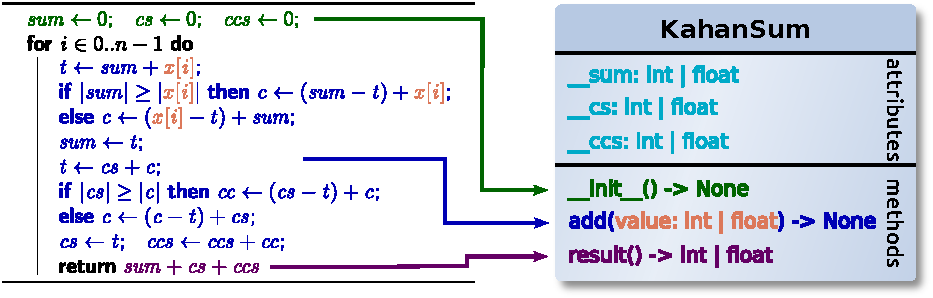
\includegraphics[width=0.85\linewidth]{\currentDir/kahanAlgorithmToClass}%
\caption{A transformation of the \citeauthor{K1965PFRORTE}-\citeauthor{B1968NSIMA}-\citeauthor{N1974REVZSES} summation algorithm specified in \cref{algo:kahanSum} to a \python\ class design. %
All state variables of the algorithm become attributes of the class. %
The initialization step setting the variables to their starting values is placed into the initializer \dunder{init}. %
The part of the algorithm body that adds numbers to the sum becomes method~\pythonil{add}. %
The final step returning the total sum can be performed at any time by querying method~\pythonil{result}.%
}%
\label{fig:kahanAlgorithmToClass}%
\afterpage{\clearpage}%
\end{figure}%
%
\gitLoadPython{classes:kahan_sum}{}{classes/kahan_sum.py}{}%
\listingPython{classes:kahan_sum}{%
An implementation of the second-order \citeauthor{K1965PFRORTE}-\citeauthor{B1968NSIMA}-\citeauthor{N1974REVZSES} summation algorithm given in \cref{algo:kahanSum}.}%
%
\gitExec{exec:classes:kahan_sum:doctest}{\programmingWithPythonCodeRepo}{.}{_scripts_/pytest_doctest.sh classes kahan_sum.py}%
\listingToolOutput{classes:kahan_sum:doctest}{%
The output of \pytest\ executing the \pglspl{doctest} for our \pythonil{KahanSum} class in module \programUrl{classes:kahan_sum}: The test succeds without error.}%
%
\gitLoadAndExecPython{classes:kahan_user}{}{classes}{kahan_user.py}{}%
\listingPythonAndOutput{classes:kahan_user}{%
Some use cases of our \citeauthor{K1965PFRORTE}-summation class from \cref{lst:classes:kahan_sum} and a comparison with \python's \pythonilIdx{sum} and the function~\pythonilIdx{fsum} from the \pythonilIdx{math} module.}{}%

However, we decide to do something else:
We want to implement it as a class \pythonil{KahanSum} that supports the creating of running sums.
It should be possible to iteratively add values to the sum and to query the current total.
Such a design is presented in \cref{fig:kahanAlgorithmToClass}.

A class has attributes and methods, right?
To figure out how we can map \cref{algo:kahanSum} to that, let's look at it more closely.
It begins by initializing the state variables \aVar{sum}, \aVar{cs}, and \aVar{ccs}.
These state variables should clearly be attributes of the objects.
In this case, their initialization would happen in the initializer \dunder{init}.
This is where we will put the code corresponding to this very first setup step of the algorithm.
And it is fairly easy to do that.

The loop in \cref{algo:kahanSum} adds one number~\aArrayIndex{\aVar{x}}{\aVar{i}} to the internal running sum at a time.
We want to implement a method \pythonil{add} that does exactly that.
It is supposed to add one new number to the internal sum and to update the first-\ and second-order error terms.
This method could then, too, be called in a loop.
The parameter \pythonil{value} of that method then takes the place of the loop variable~\aArrayIndex{\aVar{x}}{\aVar{i}}.
We can now add new numbers to this sum by invoking \pythonil{add}.

After the end of the loop, at the very end of the algorithm, the final result is computed by adding the sum variable~\aVar{sum} to the first-\ and second-order error terms~\aVar{cs} and~\aVar{ccs}.
We want to put the code computing the final result, the error-corrected sum, into a method \pythonil{result}.
Actually, when we look more closely at the algorithm, we realize that there is no reason why the result should be \emph{final}.
No state variable is changed during its computation.
If we wanted, we could query \pythonil{result} and then continue adding numbers and then query \pythonil{result} again.
This makes this a \emph{running} sum.

What we did not yet discuss are the attributes of this class.
As you can see, we should have attributes for the total sum~\aVar{sum}, the first-order error term~\aVar{cs}, and the second-order error term~\aVar{ccs}.
The values of these attributes clearly change during summation, so they won't be \pythonil{Final}.
They represent the \emph{internal} state of our sum.
They are meaningless for any outside code.
Most likely, nobody but us, who write this code, can understand their meaning.

Therefore, nobody should be able to see their values or even change them.
Because there is no reason for that.
The attributes of our class should be \emph{\inQuotes{hidden}}.
Different from the attributes~\pythonil{x} and~\pythonil{y} of our~\pythonil{Point} class, the user~(another programmer) has no business accessing the (internal) state of our sum.
Instead, the user should interact with our objects only via the methods~\pythonil{add} and~\pythonil{result}.%
%
\begin{definition}[Encapsulation]%
\emph{Encapsulation} means that all the attributes of an object can only be accessed its methods. %
Under complete encapsulation, it is impossible to read or to modify the attributes of an object in any way other than using the methods of an object. %
Encapsulation therefore allows the programmer to ensure that the state of an object can only be modified in a consistent and correct way.%
\end{definition}%
%
We want to encapsulate our objects completely.
We create the three attributes~\pythonil{__sum}, \pythonil{__cs}, and \pythonil{__ccs}.
These names are directly taken from the variable names in \cref{algo:kahanSum}, but notice the double leading underscores in front of the names.%
%
\bestPractice{doubleUnderscore}{%
Names of attributes and methods that start with a double leading underscore~(\pythonilIdx{\_\_}) are to be treated as \emph{private}~\cite{PSF:P3D:TPLR:PNM,PSF:P3D:TPT:C:PV}. %
They should not be accessed or modified from outside the class. %
All internal attributes and methods of a class that should not be exposed to the outside therefore should be named following this convention~(with two leading underscores). %
\python\ applies some internal name mangling to make such attributes harder to access from outside the class\cite{PEP8}
}%
%
In other words, nobody should access our attributes \pythonil{__sum}, \pythonil{__cs}, or \pythonil{__ccs} from the outside.
Everybody should only use our methods to access the state of our \pythonils{KahanSum}.
Sadly, like all such things, \python\ does \emph{not} enforce this{\dots}
{\dots}This naming convention is thus not an absolute protection.
It is only a very clear hint to other programmers to not touch these attributes.

We could implement the algorithm as a simple function applied to an \pythonil{Iterable} of numbers.
That would have been the most natural way to implement it.
However, we chose the class design because it allows for a much greater flexibility.
We can, of course, still use instances of our class to sum up sequences.
However, we can also use them to sum up numbers in any other way that pleases us.
We can query intermediate sums.
Or we can use multiple \pythonils{KahanSum} at the same time.
For example, if we have a stream of data, we could use two instances of \pythonil{KahanSum} to add up the data values~(in the first instance) as well as their squares~(in the second instance), which may come in handy when computing a \glslink{sampleVar}{sample variance}.

With that out of the way, we can begin the actual implementation.
A new instance of \pythonil{KahanSum} will start with all of its three summation attributes initialized to~\pythonil{0}, which is done in the initializer \dunder{init}.
We first implement the \pythonil{add} method, which corresponds to the body of the loop in \cref{algo:kahanSum}.
Looking at the algorithm, in each iteration, a value~\aArrayIndex{\aVar{x}}{\aVar{i}} is coming in and should be added to the sum.
Our \pythonil{add} method therefore has the parameter~\pythonil{value}, with the value that we want to add to the sum.
Then we just have to write down the loop body from \cref{algo:kahanSum} into \pythonil{add}.
We replace~\aVar{sum}, \aVar{cs}, \aVar{ccs}, and~\aArrayIndex{\aVar{x}}{\aVar{i}} with \pythonil{self.__sum}, \pythonil{self.__cs}, \pythonil{self.__ccs}, and~\pythonil{value}, respectively.
We write the conditional for the tweak by \citeauthor{N1974REVZSES}~\cite{N1974REVZSES} as an inline \pythonil{if...else}~statement~(see \cref{sec:inlineIfThenElse}).
For computing the absolute value~$|a|$ of a number~$a$, we can use \python's \pythonilIdx{abs}~function.
For the sake of simplicity, we can let
And that's already it.
There is nothing in the loop body of \cref{algo:kahanSum} that we cannot write down almost directly as \python\ code.

We now can place the last line of the algorithm that returns the final result of the summation into the new method~\pythonil{result}.
Obviously, it will again access the attributes \pythonil{self.__sum}, \pythonil{self.__cs}, and \pythonil{self.__ccs} in place of \aVar{sum}, \aVar{cs}, and \aVar{ccs}, respectively.
But that's it.
And we are done.
We now have translated a relatively intricate mathematical algorithm into a piece of \python\ code.
We packaged a monolithic algorithm into a \pgls{API} that can iteratively be invoked.

But does it also work?
First, we add some \pgls{doctest} to the \pgls{docstring} the module.
This \pgls{doctest} computes the sum of \pythonil{1e18 + 1 + 1e36 - 1e36 - 1e18}, which was our example from back in \cref{exec:classes:adding_floats_error}.
There, we saw that writing the sum down like this will yield~\pythonil{0.0}.
We know that the correct result should be~\pythonil{1.0}, though.
Using our \pythonil{KahanSum} class to add the elements \pythonil{[1e18, 1, 1e36, -1e36, -1e18]}, however, is \emph{supposed} to yield this correct result.
As we can see in \cref{exec:classes:kahan_sum:doctest}, it does exactly that.

In program \programUrl{classes:kahan_user} given as \cref{lst:classes:kahan_user}, we now use our new \pythonil{KahanSum} class to sum up some numbers.
We compare its result with the built-in function~\pythonilIdx{sum} and the exact summation function~\pythonilIdx{fsum} from the \pythonilIdx{math} module.
We find that all three summation algorithms can correctly add up \pythonil{[1e-15, 1e-14, 1e-13, 1e-16, 1e-12]} to~\pythonil{1.1111e-12}.
\pythonilIdx{sum} returns \pythonil{0.0} for the sum of~\pythonil{[1e+18, 1, -1e+18]} as well as for~\pythonil{[1e+36, 1e+18, 1, -1e+36, -1e+18]}.
\pythonil{KahanSum} and \pythonilIdx{fsum} both correctly compute~\pythonil{1.0} for both cases.
If we include even larger numbers and compute the sum over~\pythonil{[1e+36, 1e+72, 1e+18, -1e+36, -1e+72, 1, -1e+18]}, our \pythonil{KahanSum} returns~\pythonil{0.0} instead of the correct result~\pythonil{1.0}.
\pythonilIdx{fsum} indeed computes the correct result, whereas~\pythonilIdx{sum} is way off and returns~\pythonil{-1e18}.
Finally, we add up~\pythonil{[1, -1e-16, 1e-16, 1e-16]}.
All three methods return~\pythonil{1.0}, while the exact result would be~$1+10^{-16}$.
This number, however, cannot be represented with the datatype~\pythonil{float}.
Therefore, the results are right.

We find that \pythonilIdx{fsum} gives us the most precise result.
Our \pythonil{KahanSum} object is better than the built-in~\pythonilIdx{sum}.
This leads to two questions:%
%
\begin{enumerate}%
\item Why can our \pythonil{KahanSum} not always give us the exact results?%
\item How is \pythonil{fsum} better?%
\end{enumerate}%
%
The answer to the first question is fairly simple:
If you use only a single summation variable, as \pythonil{sum} does, then you can be precise to about 15 to 16~digits and lose all decimals beyond that.
If you have one summation variable and a first-order error term \pythonil{cs}, then you basically gain about another 15~or 16~digits for representing intermediate results more precisely.
With the second-order error term~\pythonil{ccs}, we can mantain an intermediate result with 45 to 48~digits.
This allows us to add \pythonil{1} to \pythonil{1e36} and then subtract \pythonil{1e36} again to get~\pythonil{1}.
But if we try to add \pythonil{1e72}, then we will clearly exceed this 48~digit window and the~\pythonil{1} gets lost.
So with our \pythonil{KahanSum} with two error terms, we can have intermediate results of maybe up to 48~digits.

The second question is \emph{What does \pythonilIdx{fsum} do differently?}
Actually, not very much.
It is based on the algorithm by \citeauthor{S1997APFPAAFRGP}~\cite{S1997APFPAAFRGP,H2005BFPSATFPPR}, which dynamically allocates a list of helper variables to obtain a provably exact sum~(within the result range of~\pythonil{float}).
It basically is a dynamic version of the \citeauthor{K1965PFRORTE} Sum, which uses more error term variables as needed and also drops them when they are no longer needed.
The general principle is the same, just that a list of values replaces \pythonil{cs} and \pythonil{ccs}.

Our \pythonilIdx{KahanSum} uses exactly three variables for the whole summation process.
It does not dynamically allocate more memory.
As the result, the number of steps it performs are constant for each addition.
The algorithm by \citeauthor{S1997APFPAAFRGP} implemented as \pythonilIdx{fsum} performs a variable number of steps that depends on the current length of its internal datastructure.
Thus, \pythonil{KahanSum} is indeed a very nice compromise solution, which offers higher precision than normal summing but retains the same constant memory and time complexity.

Another advantage of our \pythonil{KahanSum} over the function \pythonilIdx{fsum} is that we can use it in a more versatile fashion.
We do not need to have all values ready in an \pythonilIdx{Iterable}.
If we had a generator of a sequence of values and wanted to compute the sum of the values themselves as well as the sum of their squares, we could simply use two instances \pythonil{KahanSum} while iterating over the sequence.
With \pythonilIdx{fsum}, we would need to iterate over the sequence twice.
This may not be practical if the sequence is generated from some outside source and was too long to just store it in memory.%
%
\endhsection%
%
\hsection{Summary}%
Classes allow us to solve two problems in programming.%
%
\begin{enumerate}%
\item Wan semantically group data and the operations on the data together.%
\item We can define interfaces, i.e., \pglspl{API}, that consist of multiple operations. %
We can then create different realizations of the iterface that implement these operations in different ways.%
\end{enumerate}%
%
So far, we focussed on the first concept.
For this, we have seen two examples in this section.

We also learned about two very fundamental principles of how classes can be designed.%
\begin{enumerate}%
\item We can created immutable classes as containers for fixed information and whose attributes that does not change. %
Our \pythonil{Point} class is an example of that.%
%
\item We can also created encapsulated classes, which are classes where all access to attributes is only possible via methods of the class. %
This ensures that all state change is consistent and correct. %
The \pythonil{KahanSum} class is an example of that.%
\end{enumerate}%
%
Most classes that either actually store data or realize some behavior can be implemented in one of these two styles.
Of course, there can also by hybrid designs, e.g., classes where some attributes are \pythonil{Final} and can never change and thus are made readable for outside code without the detour over methods, while some other attributes can only be accessed and changed via methods.

Let us revisit the two example scenarios that we discussed so far.
Instances of our \pythonil{Point} class store a pair of coordinates in the two-dimensional Euclidean plane.
The operation \pythonil{distance} is inseparably linked to this data structure.
When developing it, we also learned that the first design principle mentioned above, mking objects \emph{immutable}, is a good idea.
Here, the values of the attributes of an object are set only during its initialization~(in the \dunder{init} method) and never change.
Then there can never be any confusion about the values of the attributes.
It cannot happen that one part of our process has a reference to a \pythonil{Point} variable and \inQuotes{thinks} that it's coordinates are~$(0,1)$, but some other code changed the coordinates to something else.
This cannot happen precisely because the values of the coordinates in instances of~\pythonil{Point} can never change.

If the attributes need to change, then it is often a good idea to \emph{encapsulate} them.
Encapsulation means that the attributes of an object can only be read or changed via methods of the object.
Our \pythonil{KahanSum} class is an example of this.
This class allows us to add numbers more accurately by internally keeping track of errors resulting from normal summation.
The user never gets to see these internal attributes and thus also can never modify them directly.
Instead, they are changed by passing new numbers to the \pythonil{add}~method.
Via the method~\pythonil{result}, the user can get a consistent view of the state of the summation without getting confused about its internal state.

Now, \python\ is a very lenient language.
It is very hands-off in terms what is permitted and what not.
For example, you know that \pglspl{typeHint} are only hints for tools and programmers.
The \python interpreter basically does not care about them.
It is possible to do something like \pythonil{a: str = 5}.
This leniency also concerns both design principles above.

Attributes and variables are made \inQuotes{immutable} by annotating them with the \pgls{typeHint} \pythonilIdx{Final}.
Since this, again, is only a \pgls{typeHint}, it is just information for the programmer and for tools.
The \python\ interpreter ignores it.
We can do \pythonil{a: Final[int] = 5} and then \pythonil{a = 6} without punishment.
Similarly, marking attributes as private by using names starting with a double underscore~(\pythonilIdx{\_\_}) does not actually make them private.
The \python\ interpreter applies some name mangling~\cite{PEP8} to make them harder to access, but a crafty programmer can still read and write them.
Tools like \mypy, however, will also spot such misconduct.

\python\ places the responsibility into our hands to properly adher to standards and coding rules.
But it does not enforce such behavior.

In the next section, we will see how inheritance of classes in \python\ can be used to implement \pglspl{API}, which is the second big use-case of classes.%
\endhsection%
%
\FloatBarrier%
\endhsection%
